\chapter{L-simulaci\'on en acci\'on}
\label{sec:intro_logica}

De acuerdo a lo que queremos permitir en una ER, tendremos un lenguaje asociado, el cual pertenecer\'a a alguna l\'ogica. En este cap\'itulo se explica como partiendo de \FOL podemos ir restringiendo la l\'ogica y con ello el lenguaje, siendo la complejidad un tema interesante abordar, ya que por ejemplo sistemas de tiempo real necesitan conseguir ER r\'apidamente, daremos las complejidad de las distintas l\'ogicas, y veremos que l\'gica aplica a cada uno de los algoritmos del \'area



\section{Seleccionando el lenguaje}





Intuitivamente, dado un lenguaje l\'ogico $\+L$ decimos que un objeto $u$ en un modelo
$\+M_1$ es similar en $\+L$ a otro objeto
 $v$ en el model $\+M_2$ para cualquier $\+L$-f\'ormulas que son satisfechas por $u$ tambi\'en son satisfechas por $v$. Formalmente,
%let $\+L$ stand for any of the languages discussed so far, and
Sea $\+M_1 = \tup{\Delta_1, \interp{\cdot}_1}$ y $\+M_2 = \tup{\Delta_2, \interp{\cdot}_2}$ 2 modelos relacionales con $u \in \Delta_1$ y $v \in \Delta_2$; seguimos la terminolog\'ia de~\cite{areces08} y decimos que
\emph{$u$ es $\+L$-similar a $v$}  (notaci\'on $u \simil{\+L} v$) si para toda $\gamma \in \+L$, $u \in \interp{\gamma}_1$ implica
$v \in \interp{\gamma}_2$. Es facil mostrar que
$\+L$-similaridad es reflexiva para todo $\+L$, y simm\'etrica  para languajes que contienen negaci\'on.


Observe que la $\+L$-similitud captura la noci\'on de ``capacidad de identificar en $\+L$''. Si tomamos $\+M_1$ y $\+M_2$ a ser del mismo modelo, un objeto $u$ en el modelo identificarse un\'ivocamente en $\+L$ si no hay ning\'un objeto $v$ diferente de $u$ tal que $u \simil{\+L} v$. En otras palabras, si hay dos objetos $u$ y $v$ en un modelo $\+M$  tal que
$u \simil{\+L} v$, entonces el problema $\+L$-GRE con entrada de $\+M$ y destino $T=\{u\}$ no tendr\'a \'exito ya que para todas las f\'ormulas $\gamma \in L$ tenemos que $\{u,v\} \subseteq \interp{\gamma} \not = \{u\}$.

La noci\'on de $\+L$-similitud entonces, nos permite manejar el problema de  $\+L$-GRE.
Por otra parte, podemos reformular esta de noci\'on de una manera estructural, por lo que no lo hacemos
que considerar en muchos $\+L$-f\'ormulas infinitamente decidir si $u$ es $\+L$- similar a $v$. Podemos reinterpretar $\+L$-similitud en t\'erminos de nociones de teor\'ia de modelos estandares
como isomorfismos o bisimulaciones que describen las propiedades estructurales del modelo. Dados dos modelos$\tup{\Delta_1, \interp{\cdot}_1}$ and $\tup{\Delta_2,
\interp{\cdot}_2}$, considere las siguiente
propiedades de una relaci\'on binaria ${\sim} \subseteq \Delta_1 \times \Delta_2$ (cf.~Convention~\ref{conv:signature}):
\smallskip 

\newcommand{\simdef}[2]{\noindent\ \ #1\hfill:\ \parbox[t]{.87\textwidth}{#2}\par}

\simdef{$\atomL$}{If $u_1{\sim} u_2$, entonces $u_1 \in \interp{p}_1 \Rightarrow u_2 \in \interp{p}_2$}
\simdef{$\atomR$}{If $u_1{\sim} u_2$, entonces $u_2 \in \interp{p}_2 \Rightarrow u_1 \in \interp{p}_1$}
\simdef{$\zig$}{If $u_1{\sim} u_2$ y $(u_1,v_1) \in \interp{r}_1$, entonces $\exists v_2$ s.t.\ $v_1{\sim}v_2$
  y $(u_2,v_2) \in \interp{r}_2$}
\simdef{$\zag$}{If $u_1{\sim}u_2$ y $(u_2,v_2) \in \interp{r}_2$, entonces $\exists v_1$ s.t.\ $u_1{\sim}v_1$ y
 $(u_1,v_1) \in \interp{r}_1$}
\simdef{$\injL$}{$\sim$ es una funci\'on inyectiva (cuando es restringida a su dominio)}
\simdef{$\injR$}{$\sim^{-1}$ es una funci\'on inyectiva (cuando es restringida a su dominio)}
\smallskip

Diremos que una relacion binaria no-vac\'ia $\sim$ es una 
\emph{$\+L$-simulation} cuando satisface las propiedades indicadas
en la Tabla~\ref{tab:simuls}. Por ejemplo, una relacion binaria no-vac\'ia que satisface $\atomL$, y $\zig$ es una $\EL$-simulation, como es indicado en fila~4 de la Tabla~\ref{tab:simuls}. M\'as a\'un, diremos que un objeto
\emph{$v$ $\+L$-simulates $u$} (notaci\'on $u \simul{\+L} v$) si hay una relaci\'on $\sim$ que satisface el correspondiente propiedad tal que
$u \sim v$. El siguiente es un resultado fundamentar del modelo-teor\'etico  result:%~\cite{ebbi:math96,KR99,BRV01}

\begin{table}[t]

\begin{tabular}{|l|l|cccccc|l|}
\hline
  $\+L$ & Descripci\'on &$\atomL$ & $\atomR$ & $\zig$ & $\zag$ & $\injL$ & $\injR$ & Comp.\\
  \hline
  $\FOL$ & (l\'ogica de primer orden)  & $\times$ & $\times$ & $\times$ & $\times$ & $\times$ & $\times$ & NP\\ \hline
  $\EPFOL$ & ($\FOL$ sin negaci\'on) & $\times$ & & $\times$ && $\times$ & & NP\\ \hline 
  $\ALC$   & ($\FOL$ sin desigualdad) & $\times$ & $\times$ & $\times$ & $\times$&& & P\\ \hline
  $\EL$   & ($\ALC$ sin negaci\'on) & $\times$ & &  $\times$ & & & &P\\ \hline
	$\ELUNEG$ & ($\EL$ m\'as disyunci\'on y  & $\times$ & $\times$ &  $\times$ & & & &P\\ 
	&negaci\'on proposicional)&&&&&&&\\ \hline
  $\ELAN$ & ($\EL$ con negaci\'on & $\times$ & $\times$ &  $\times$ & & & &P\\ 
	&proposicional) &&&&&&& \\ \hline
	$\PL$ & ($\ALC$ sin existencial --- & $\times$ & $\times$ & & & & &P\\ 
	&conj. dis. neg. prop.)&&&&&&&\\ \hline
	$\CL$ & (prop. conj. sin negaci\'on)& $\times$ &  &  & & & &P\\ 
	
\hline	
\end{tabular}

\caption{$\+L$-simulaciones para varios lenguajes l\'ogicas.}\label{tab:simuls}
\end{table}


Una l\'ogica sim\'etrica cumple  $\atomL$ y $\atomR$ como se ve en la Tabla \ref{tab:simuls}. 


\begin{table}[h!]
\begin{tabular}{l|l}
  Algoritmo de GER & Variante de L\'ogica de Descripci\'on (DL)\\
  \hline
	  Full brevity & $\CL$ (proposicionales y conjunciones --- sin negaci\'on) \\
		Heuristica Greedy & $\CL$ (proposicionales y conjunciones --- sin negaci\'on) \\
  Incremental - Dale and Reiter (1995) & $\CL$ (proposicionales y conjunciones --- sin negaci\'on) \\
  GRAPH - van Deemter (2002) & $\PL$ (f\'ormulas conjuntivas, disjuntivas, negativas prop. \\
														& ---l\'ogica proposicional idem $\ALC$ sin existencial)\\
  Relacional - Dale and Haddock (1991)   & $\EL$ (Conjunciones de f\'ormulas, existenciales de f\'ormulas, \\
	& y proposicionales)\\
  Kelleher and Kruijff (2006)   & $\EL$ \\
  Gardent (2002) & \ELUNEG ($\EL$ m\'as disyunci\'on y negaci\'on proposicional)\\
\end{tabular}

\caption{Algoritmos y sus l\'ogicas asociadas.}\label{tab:simuls}
\end{table}
\textcolor{blue}{
\ALC tiene negacion de formulas, conjunciones y existenciales, proposicionales
}
\begin{theorem} \label{thm:simulation}
If  $\+M_1 = \tup{\Delta_1, \interp{\cdot}_1}$ and $\+M_2 =
\tup{\Delta_2, \interp{\cdot}_2}$ son modelos finitos, $u \in
\Delta_1$ and $v \in \Delta_2$, then $u \simil{\+L} v$ iff $u
\simul{\+L} v$ (for $\+L \in \cset{\FOL,\EPFOL,\ALC,\EL,\ELAN}$).
\end{theorem}
%\begin{proof}
Algunos resultados son bien conocidos: $\simul{\FOL}$ es isomorfismo en
grafos etiquetados~\cite{ebbi:math96}; $\simul{\ALC}$ corresponde a la
noci\'on de bisimulaci\'on~\cite[Def.~2.16]{BRV01}; $\simul{\EL}$ es una
simulaci\'on definida en~\cite[Def.~2.77]{BRV01}. Los restantes son variaciones de estos.
%\end{proof}


Therefore, on finite models\footnote{Finiteness is not the weakest hypothesis,
but it is enough for our development.} simulations capture exactly the notion of similarity.
The right to left implication does not hold in general on infinite
models.

$\+L$-simulations allow us to determine, in an effective way,
when an object is indistinguishable from another in a given model with respect to $\+L$.

For example, we can verify that $a \simul{\EL} b$ in the model of
Figure~\ref{fig:cat-dog-1} (the relation ${\sim} = \{(a,a), (a, b) \}
%\cup\{ (x,x) \mid x \in \Delta\}
$ satisfies $\atomL$ and $\zig$).
Using Theorem~\ref{thm:simulation}
we conclude that there is no \EL-description for $a$, since for any \EL-formula $\gamma$,
if $a\in\interp{\gamma}$, then $b\in\interp{\gamma}$.
Observe that $b \not\simul{\EL} a$, since
(again applying Theorem~\ref{thm:simulation}), $b\in\interp{\aSmall(x)}$ but
$a\notin\interp{\aSmall(x)}$.
%
If one chooses a language richer than $\EL$, such as $\ELAN$, one may be
able to describe $a$: take, for instance the $\ELAN$-formula
$\nDog(x)\wedge\lnot\aSmall(x)$.


As we will discuss in the next section, simulation gives us an
efficient, computationally feasible approach to the $\+L$-GRE
problem. Algorithms to compute many kinds of $\+L$-simulations are
well known (see, \cite{H71,areces08,HHK95,DPP03}), and for many
languages  (e.g., \ALC, \ALC with inverse relations,  \ELAN and \EL)
they run in polynomial time (on the other hand, no polynomial
algorithm for \FOL- or \EPFOL-simulation is known and even the exact
complexity of the problem in these cases is open
\cite{gare:comp79}).

\section{GRE via Simulator Sets}\label{sec:simulation}

En esta secci\'on discutiremos como resolver el problema $\+L$-GRE
usando simulation. Dado a model $\+M = \tup{\Delta,
\interp{\cdot}}$, Theorema~\ref{thm:simulation} nos dice que si 2 elementos distintos $u$ y $v$ en $\Delta$ son tales que $u
\simul{\+L} v$ entonces para toda $\+L$-f\'ormula que es verdadera para $u$ es tambi\'en verdadera para $v$. No hay f\'ormula en $\+L$ que pueda identificar un\'ivocamente a $u$. Desde esta perspectiva, conociendo cuando el modelo contiene un elemento que es $\gL$-similar pero distinto de $u$ es
equivalente a decidir hay una $\+L$-RE for $u$.


Asumamos un lenguaje fixo $\+L$ y un modelo $\+M$.  Supongamos que queremos referirnos a un elemento $u$ del dominio de $\+M$. Queremos computar \emph{simulator set} de $u$ definidas como
$\simset_{\+L}^{\+M}(u) = \cset{v \in \Delta \mid u \simul{\+L} v}$.
Cuando un modelo $\+M$ is clear from the context, we just write
$\simset_{\+L}$.
 If $\simset_{\+L}^{\+M}(u)$ no es singleton $\cset{u}$,
el problem $\+L$-GRE con target $\{u\}$ en $\+M$ fallar\'a.

\iffullversion
Es facil de ver que la union de 2 $\+L$-simulations es
es tambi\'en una $\+L$-simulation. Podemos entonces definir el \emph{maximal
auto $\+L$-simulation} (notaci\'on, $\simmax_{\+L}$) sobre un modelo $\+M$ como la union de todos los
auto $\+L$-simulations sobre $\+M$. Ya que
$\simset_{\+L}(u) = \cset{v \mid u \simmax_{\+L} v}$, un algoritmo
para computar $\simmax_{\+L}$ tambi\'en computa $\simset_{\+L}(u)$.
\else
\fi

\iffullversion
If $P$ es reflexiva y transitiva entonces tambi\'en lo es $\simmax_P$. En
particular, $\simmax$ es reflexiva y transitiva.
\fixme{Are reflexivity and transitivity important? Check.}
\else
\fi



Un algoritmo es dado en~\cite{HHK95} para computar $\simset_{\ELAN}(v)$ para cada
elemento $v$ de un modelo dado finito
$\+M=\tup{\Delta,\interp{\cdot}}$
%\footnote{%
%  Actually the algorithm proposed in \cite{HHK95} is over labeled graphs, but
%  it can be adapted to compute $\simset_{\ELAN}$ by
%  appropriately labeling the model.%
%}
en tiempo $O(\size{\Delta}\times\size{{\interp{\cdot}}})$.
Intuitivamente, este algoritmo
define $S(v)$ como un conjunto de candidatos para simuolar $v$ y
sucesivamente refina este borrando aquellos los cuales falla en simular $v$.
%Since we never put new vertices into $\simset(v)$, all the deletions
%from $\simset(v)$ are permanent.
Al final, $S(v)=\simset_\ELAN(v)$. El algoritmo puede ser adaptado para
computar $\simset_\+L$ para cualquier otro languaje $\+L$. En particular,
lo podemos usar para computar $\simset_\EL$ en tiempo polinomial which will
give us the basic algorithm for establishing an upper bound to the
complexity of the \EL-GRE problem --this will answer an open
question of~\cite{areces08}. The pseudo-code is shown in
Algorithm~\ref{alg:schematic-gen-sim}, which uses the following
notation: $\+P$ is a fixed set of unary relation symbols,  for $v\in
\Delta$, let $\unary(v)=\{p\in\+P\mid v\in\interp{p}\}$ and let also
$\su{r}{v}=\{u\in\Delta\mid(v,u)\in\interp{r}\}$ for $r$ a binary
relation symbol.


\section{Bisimulaci\'on}
\label{sec:bisimulacion}

%Este algoritmo fue propuesto por %\cite{}

La idea es transformar el problema de GER al problema de computar una f\'ormula de l\'ogicas para la descripci\'on (DL) cuyos elementos que satisfagan la f\'ormula sea el target.% (o los elementos targets, en el caso de querer dar una ER para plurales aprovechando que una f\'ormula describe un conjunto que puede contener m\'as de un elemento).\\

A continuaci\'on daremos una introducci\'on a las l\'ogicas para la descripci\'on \alc y \el. Explicaciones m\'as detalladas sobre \alc y \el se ver\'an en el Cap\'itulo \ref{sec:intro_logica}.

\emph{F\'ormulas} (o \emph{conceptos}) $\varphi$ de $\alc$ son generadas por la siguiente gram\'atica:
$$
\varphi,\varphi' ::= \top \mid p \mid \neg \varphi \mid \varphi \sqcap \varphi'
\mid \exists R. \varphi
$$
donde $p$ es el conjunto de los s\'imbolos proposicionales \prop y $R$ es el de los s\'imbolos relacionales \rel. $\el$ es la parte sin negaci\'on de $\alc$.\\

Las f\'ormulas de ambos $\alc$ y $\el$ son interpretadas en modelos relacionales de primer orden $\gM = (\Delta,\interp{\cdot})$ donde
$\Delta$ es un conjunto no vac\'io y $\interp{\cdot}$ es una funci\'on de interpretaci\'on tal que:
$$
\begin{array}{ccl}
\interp{p} & \subseteq & \Delta  \mbox{ para $p \in \prop$}\\
\interp{R} & \subseteq & \Delta \times \Delta  \mbox{ para $R \in \rel$}\\
\interp{\neg \varphi} & = & \Delta - \interp{\varphi}\\
\interp{\varphi \sqcap \varphi'} & = & \interp{\varphi} \cap \interp{\varphi'}\\
\interp{\exists R.\varphi} & = & \{i \mid \mbox{para alg\'un } i', (i,i') \in \interp{R}\\
& & \mbox{ e } i' \in \interp{\varphi} \}.\\
\end{array}
$$

\begin{figure}[ht]
\begin{center}
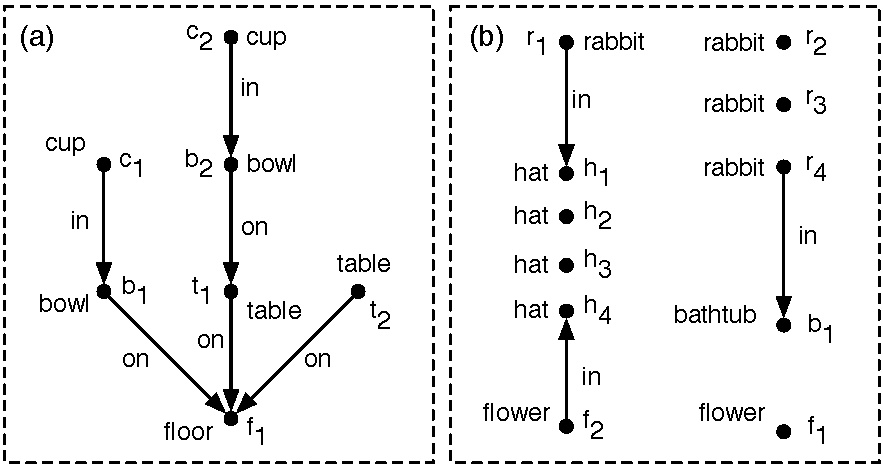
\includegraphics[width=8.5cm]{figures/pic-dale-haddock.pdf}\\[0pt]
\caption{}
\label{fig:dale-haddock}
\end{center}
\end{figure}


Cada f\'ormula de una descripci\'on l\'ogica denota un conjunto de objetos del dominio; por lo tanto podemos usar tales f\'ormulas para describir conjuntos. Por ejemplo en el modelo de la Figura.~\ref{fig:dale-haddock}b, la f\'ormula
$\mathsf{flower}$ denota el conjunto $\{f_1,f_2\}$; La f\'ormula
$\mathsf{flower} \sqcap \exists \mathsf{in}.\mathsf{hat}$ denota
$\{f_2\}$; y la f\'ormula $\mathsf{flower} \sqcap \neg
\exists \mathsf{in}.\mathsf{hat}$ denota $\{f_1\}$.\\

\textcolor{blue}{no se si dejar este ejemplo, o cambiarlo por uno es espa\~nol}

Hay muchas otras l\'ogicas de descripci\'on (DL) en la literatura por ejemplo 

$\mathcal{CL}$ (\el\ sin el cuantificador existencial, es decir solo conjunciones at\'omicas); $\mathcal{PL}$ (\alc\ l\'ogica propocisional); y
$\mathcal{ELU}_{(\neg)}$ (\el\ m\'as disjunci\'on y negaci\'on at\'omica).\\

Usaremos una noci\'on de preservaci\'on de f\'ormulas que llamaremos
\emph{similaridad}. Para cualquier DL $\gL$, diremos que un individual $i$ es \emph{\gL-similar} a $i'$ en un modelo dado $\gM$
si para cualquier f\'ormula $\varphi \in \gL$ tal que $i \in
\interp{\varphi}$, tambi\'en tenemos que $i' \in \interp{\varphi}$.\\
Equivalentemente, no hay $\gL$-f\'ormula que se mantenga para $i$ pero no para
$i'$.  Diremos que el \emph{\gL-conjunto de similaridad} de alg\'un individual
$i$ es el conjunto de todos los individuales a los cuales $i$ es \gL-similar.\\

Notar que la similaridad no es necesariamente una relaci\'on sim\'etrica: Por ejemplo:$f_1$ es \el-similar a $f_2$ en
Figura~\ref{fig:dale-haddock}b, pero $f_2$ no es \el-similar a $f_1$
(satisface la f\'ormula $\exists \mathsf{in}.\mathsf{hat}$ y $f_1$
no la satisface).  De todas maneras, \alc-similaridad es una relaci\'on sim\'etrica porque
el languaje contiene negaci\'on; y en consecuencia, $f_1$ no es \alc-similar
a $f_2$ porque este tampoco satisface $\neg \exists
\mathsf{in}.\mathsf{hat}$.  Porque \alc\ es m\'as expresivo que \el,
esto es, para alg\'un individual $a$ es posible ser \el-similar pero
no \alc-similar a alg\'un individual $b$, pero no viceversa.\\



%\textcolor{blue}{SACAR ESTO... poner quizas en la introduccion o en primer capitulo. Las ER que involucran relaciones han recibido m\'as atenci\'on recientemente;
%especialmente en el contexto de las expresiones referenciales espaciales en generaci\'on (por ejemplo,~\cite{kelleher06:increm}), donde es particularmente natural utilizar expresiones que implican relaciones espaciales, tales como ``la esfera en la parte superior del cubo''. Sin embargo, el algoritmo cl\'asico por~\cite{dale91:gener} ha demostrado ser incapaz de generar ER satisfactorias en la pr\'actica (v\'ease el an\'alisis sobre el~\emph{cabinet corpus} en~\cite{viethen06:_algor_for_gener_refer_expres}). Adem\'as, el Dale y Haddock algoritmo y muchos de sus sucesores (tales como~\cite{kelleher06:increm}) son vulnerables a el problema de la \emph{regresi\'on infinita}, donde el algoritmo entra en un bucle infinito, saltando hacia atr\'as y hacia adelante entre las descripciones para dos individuos emparentados, como en `` el libro sobre la mesa que soporta una libro sobre la mesa \ldots ''}

%REs involving relations have received increasing attention recently;
%especially in the context of spatial referring expressions in situated
%generation (e.g., \cite{kelleher06:increm}),
%where it is particularly natural to use expressions involving spatial
%relations such as ``the ball on top of the cube.''  However, the
%classical algorithm
%by~\cite{dale91:gener} was shown to be
%unable to generate satisfying REs in practice (see the analysis over
%the \emph{cabinet corpus}
%in~\cite{viethen06:_algor_for_gener_refer_expres}).  Furthermore, the
%Dale and Haddock algorithm and many of its successors (such
%as~\cite{kelleher06:increm}) are vulnerable to
%the problem of \emph{infinite regress}, where the algorithm enters an
%infinite loop, jumping back and forth between descriptions for two
%related individuals, as in ``the book on the table which supports a
%book on the table \ldots''

%\cite{arec2:2008:Areces,arec:usin11} have proposed low complexity
%algorithms for the generation of relational REs
%%(including references to sets) 
%that eliminate the risk of infinite regression.  These algorithms are
%based on variations of the partition refinement algorithms
%of~\cite{paig:thre87}.  The information provided by a given scene
%is interpreted as a relational model whose objects are classified into
%sets that fit the same description.  This classification is
%successively \emph{refined} till the target is the only element
%fitting the description of its class.  The existence of an ER depends
%on the information available in the input scene, and on the expressive
%power of the formal language used to describe elements of the
%different classes in the refinement.


\cite{arec2:2008:Areces,arec:usin11} han propuesto algoritmos de baja complejidad
 para la generaci\'on de ER relacionales que eliminan el riesgo de regresi\'on infinita. Estos algoritmos son
basados en variaciones de los algoritmos de refinamiento de particiones
de~\cite{paig:thre87}. La informaci\'on proporcionada por una escena dada
se interpreta como un modelo relacional cuyos objetos se clasifican en
conjuntos que se adaptan a la misma descripci\'on. Esta clasificaci\'on es
sucesivamente \emph{refinada} hasta que el target es el \'unico elemento
en la clase. La existencia de una ER depende
de la informaci\'on disponible en la escena de entrada, y del poder expresivo
del lenguaje formal utilizado para describir los elementos de las
diferentes clases en el refinamiento.\\

%Refinement
%algorithms %presented in~\cite{arec2:2008:Areces,arec:usin11}
%effectively compute REs for all individuals in the domain, at the same
%time. The algorithms always terminate returning a formula of the
%formal language chosen that uniquely describes the target (if the
%formal language is expressive enough to identify the target in the
%input model).
%\cite{arec2:2008:Areces}
%show that the refinement algorithm using the description language \el  is capable of generating 67\% of 
%the relational REs in the~\cite{viethen06:_algor_for_gener_refer_expres} dataset, when all possible orders of the relations in the domain are considered. This is in sharp contrast with the analysis 
%done in~\cite{viethen06:_algor_for_gener_refer_expres} over the cabinet corpus, of algorithms based in Dale and Reiter's original proposal.    

%Los algoritmos de refinamiento
% presenta en~\cite{arec 2:2008:Areces, arec:usin11}
%calculan efectivamente ER para todos los objetos en el dominio, al mismo
%tiempo. Los algoritmos siempre terminan devolviendo una f\'ormula del
%lenguaje formal elegido que describe un\'{i}vocamente el target (si el
%lenguaje formal es suficientemente expresivo para identificar el target en el
%modelo de entrada).\\

%Refinement algorithms for GER are based on the following basic idea:
%given a scene $S$, the objects appearing in $S$ are successively
%classified according to their properties into finer and finer
%classes. A description (in some formal language $\mathcal{L}$) of each
%class is computed every time a class is refined. The procedure always
%stops when the set of classes stabilizes, i.e., no further refinement
%is possible with the information available in the scene\footnote{Of
%  course, if we are only interested in a referring expression for a
%  given target we can stop the procedure as soon as the target is the
%  only element of some of the classes.}.  If the target element is in
%a singleton class, then the formal description of that class is a
%referring expression; otherwise the target cannot be unequivocally
%described (in 


%It is clear that a scene can be encoded in different ways as a
%relational model (for example in \ref{figure22}, we could argue that
%$e_1$ is also \emph{leftof} $e_2$, not considered because they are no
%touching). The algorithm assumes that these issues have been resolved
%and that the model encodes a suitable representation of the scene we
%want to describe.  Moreover, we will assume that all relations are
%\emph{binary}.  We will not consider relations of arity greater than
%two (relations of higher arity can be encoded as binary relations via
%reification, if necessary).

\begin{figure}[ht]
%\begin{minipage}[b]{0.45\linewidth}
%\centering
\begin{center}
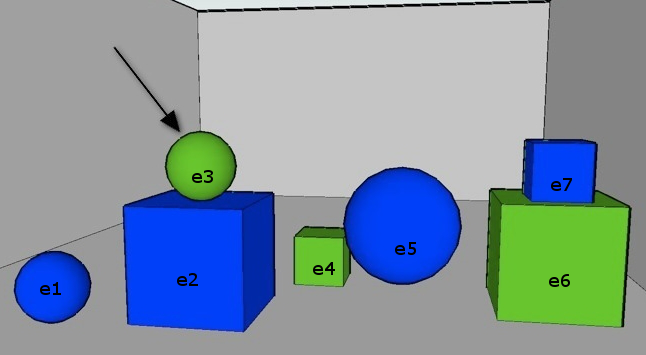
\includegraphics[width=0.5\textwidth]{images/3b.png}
\caption{Contexto de ejemplo}\label{GRE3D7-stimulus-cap2}
%\end{minipage}
\end{center}
\end{figure}

%\textcolor{blue}{hice mas grande la figura porque no se leian, como la pase a espaniol y se me fue al pie, no se porque}
%\hspace*{-0.35cm}
\begin{figure}[ht]
\begin{center}
%\begin{minipage}[b]{0.5\linewidth}
%\centering
\begin{tikzpicture}
  [
    n/.style={circle,fill,draw,inner sep=3pt,node distance=2.6cm},
    aArrow/.style={->, >=stealth, semithick, shorten <= 2pt, shorten >= 2pt},
  ]
 \node[n,label=above:$e_1$,label=below:{
    \relsize{-1}$\begin{array}{c}
      \nLeft\\[-2pt]
      \nSmall\\[-2pt] 
      \nBlue \\[-2pt] 
      \nBall\end{array}$}] (a) {};

 \node[n,label=above:$e_2$,label=below:{
    \relsize{-1}$\begin{array}{c}
      \nLeft\\[-2pt]
      \nBig\\[-2pt] 
      \nBlue\\[-2pt] 
      \nCube\end{array}$}, right of=a] (b) {};

 \node[n,label=below:$e_3$,label=above:{
    \relsize{-1}$\begin{array}{c}
      \nTop\\[-2pt]
      \nLeft\\[-2pt]
      \nSmall\\[-2pt] 
      \nGreen\\[-2pt] 
      \nBall\end{array}$}, above of=b] (c) {};

 \node[n,label=above:$e_4$,label=below:{
    \relsize{-1}$\begin{array}{c}
      \nSmall\\[-2pt] 
      \nGreen\\[-2pt] 
      \nCube\end{array}$}, right of=b] (d) {};

 \node[n,label=above:$e_5$,label=below:{
    \relsize{-1}$\begin{array}{c}
      \nBig\\[-2pt] 
      \nBlue\\[-2pt] 
      \nBall\end{array}$}, right of=d] (e) {};

 \node[n,label=above:$e_6$,label=below:{
    \relsize{-1}$\begin{array}{c}
      \nBig\\[-2pt] 
      \nGreen\\[-2pt] 
      \nCube\end{array}$}, right of=e] (f) {};

 \node[n,label=below:$e_7$,label=above:{
    \relsize{-1}$\begin{array}{c}
      \nTop\\[-2pt]
      \nSmall\\[-2pt] 
      \nBlue\\[-2pt] 
      \nCube\end{array}$}, above of=f] (g) {};

 \draw [aArrow,bend right=90] (b) to node[auto,swap]{\relsize{-1}$\nBelow$} (c);
 \draw [aArrow,bend right=90] (c) to node[auto,swap]{\relsize{-1}$\nOntop$} (b);

 \draw [aArrow,bend right=70] (d) to node[auto,swap]{\relsize{-1}$\nLeftof$} (e);
 \draw [aArrow,bend right=70] (e) to node[auto,swap]{\relsize{-1}$\nRightof$} (d);

 \draw [aArrow,bend right=90] (f) to node[auto,swap]{\relsize{-1}$\nBelow$} (g);
 \draw [aArrow,bend right=90] (g) to node[auto,swap]{\relsize{-1}$\nOntop$} (f);

 \draw[dotted] (-.6,-2.2) rectangle (12.5,5.3);

 \end{tikzpicture}
\caption{Modelo relacional del Contexto \ref{GRE3D7-stimulus-cap2}}
\label{GRE3D7-stimulus-graph}
%\end{minipage}
\end{center}
\end{figure}

Algoritmos de refinamiento para GER se basan en la siguiente idea b\'asica:
dada una escena $S$, los objetos que aparecen en $S$ son sucesivamente
clasificados de acuerdo con sus propiedades en clases m\'as y m\'as finas. 
Una descripci\'on (en alg\'un lenguaje formal de $\mathcal{L}$) de cada
clase se calcula cada vez que una clase es refinada. El procedimiento siempre
se detiene cuando el conjunto de clases se estabiliza, es decir, no se puede hacer m\'as refinamiento
con la informaci\'on disponible en la escena \footnote{Por supuesto, si s\'olo estamos interesados en una expresi\'on referencial de un objeto dado, se puede detener el procedimiento en cuanto el objetivo es el
   \'unico elemento de alguna de las clases.}

Si el elemento target est\'a en
una clase singleton, entonces la descripci\'on formal de esa clase es un
expresi\'on referencial; de lo contrario el target no puede ser un\'{i}vocamente
descripto (en $\mathcal{L}$).

Est\'a claro que una escena puede ser codificada en diferentes formas como un
modelo relacional (por ejemplo, en \ref{GRE3D7-stimulus-cap2}, podr\'{i}amos argumentar que
$e_1$ es tambi\'en \emph{leftof} $e_2$, pero no lo consideramos porque no se estan 
tocando en la imagen). El algoritmo asume que estas cuestiones se han resuelto y que el modelo codifica una representaci\'on adecuada de la escena que
queremos describir. Por otra parte, vamos a suponer que todas las relaciones son
\emph{binarias}. No vamos a considerar las relaciones de aridad mayor que
dos (relaciones de mayor aridad pueden codificarse como relaciones binarias v\'{i}a
reificaci\'on, si es necesario).

%On termination, the algorithm computes what are called the
%$\mathcal{L}$-similarity classes of the input model $\gM$.
%Intuitively, the referring expression ``\textsf{ball}'' and ``\textsf{cube}''  are more specific and then contain more information than $\top$.


Tras la resoluci\'on, el algoritmo calcula lo que se llama la
$\mathcal{L}$ - clases de semejanza del modelo de entrada de $\gM$.\\

%There is many $\mathcal{L}$, we will name $\alc$ and $\el$

%ACA VOY A PONER gramatica para generar... ALC y EL no quedaria bien aca, hay que ver lo agregamos antes o no hace falta
%In what follows, we use formulas of the $\el$ description logic
%language
En lo que sigue, se utilizan f\'ormulas de la descripci\'on de la l\'ogica $\el$
~\cite{baad:desc03} para describir las clases de refinamiendo
\footnote{N\'otese, sin embargo, que el lenguaje formal particular usado es
   independiente del algoritmo principal, y diferentes funciones
  add$_{\mathcal{L}}$($\varphi$,\RE) se pueden utilizar dependiendo
   de la l\'ogica en cuesti\'on.}. como se discuti\'o 
en~\cite{arec2:2008:Areces}, 
este lenguaje es adecuado para describir
RE conjuntivas y relacionales, que son lo que encontramos en los corpus.

  La entrada al algoritmo ser\'a un modelo $\mathcal{M} =
 \tup{\Delta, \interp{\cdot}}$, donde $\Delta$ es el dominio no vac\'io de objetos de la imagen,
 $\interp{\cdot}$ es una funci\'on de interpretaci\'on que asigna a todas las propiedades de la escena su extensi\'on.
 Por ejemplo, la escena mostrada en la Figura~\ref{GRE3D7-stimulus-cap2} podr\'ia ser representada por el modelo
 $\gM=\tup{\Delta,\interp{\cdot}}$ mostrado en la 
 Figura~\ref{GRE3D7-stimulus-graph}; donde+- $\Delta =
 \{e_1,\ldots,e_7\}$, e $\interp{\textsf{red}}$ is $\{e_2, e_4, e_5,
 e_7\}$.

Se llama extensi\'on de una f\'ormula al conjunto de objetos que la hacen v\'alida.

$\top$ es una f\'ormula que representa la descripci\'on m\'as general, cuya
interpretaci\'on incluye todos los elementos del modelo. Se podr\'ia realizar
como la ER con el sustantivo
``\textsf{cosa}''. Decimos que una f\'ormula es
\emph{subsumida} por otras f\'ormulas, cuando su extensi\'on puede ser cubierta por la
union de las extensiones de las otras f\'ormulas. Por ejemplo, en la
Figura~\ref{GRE3D7-stimulus-cap2}, $\top$ es subsumida por ``\textsf{esfera}'' y
``\textsf{cubo}'', porque $\interp{\top}$ = $\interp{\textsf{esfera}}
\cup \interp{\textsf{cube}}$.
%= $\{e_2, e_4, e_6, e_7\}$, it is $\{e_1, e_2, e_3, e_4, e_5, e_6, e_7\}$ = $\{e_1, e_3, e_5\} \cup \{e_2, e_4, e_6, e_7\}$. 
Intuitivamente la f\'ormula ``\textsf{cubo}'' o ``\textsf{esfera}'' tienen m\'as informaci\'on que $\top$, para cada elemento de $\top$, hay una f\'ormula que d\'a m\'as informaci\'on, digamos ``\textsf{cubo}'' es m\'as informativa que ``\textsf{cosa}''.\\

%In the following we will explain an example of execusion of the
%algorithm shown in Figure
%A continuaci\'on vamos a explicar un ejemplo de ejecusi\'on del
%algoritmo mostrado en la Figura~\ref{algoritmoOriginal} considerando la l\'ogica 
%$\el$ como language. Este algoritmo fue presentado en
%~\cite{arec2:2008:Areces}.
%
%\begin{figure}[h!]
%\begin{center}
%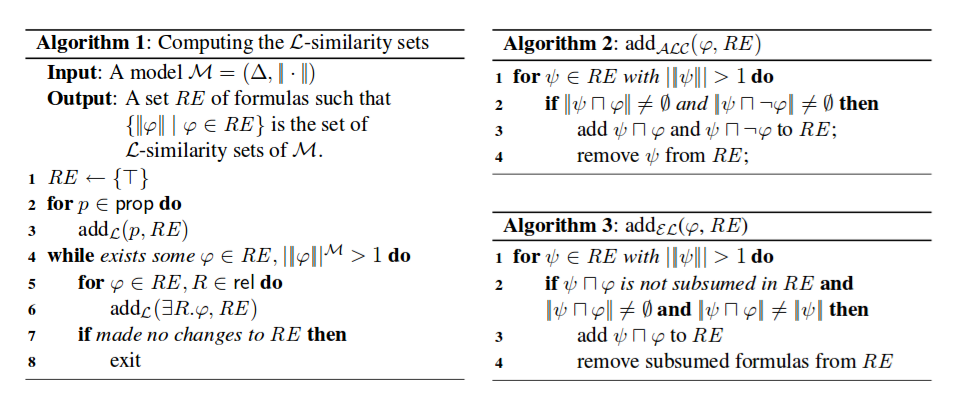
\includegraphics[width=\textwidth]{images/algoritmoOriginal.png}
%\end{center}
%\vspace*{-2em}
%\caption{Algoritmo para GER con l\'ogicas de descripci\'on}
%\label{algoritmoOriginal}
%\end{figure}

%\subsection{Ejemplo de ejecuci\'on}
%
%
%
%\textcolor{blue}{no se si poner aca un ejemplo, si poner el texto y las im\'agenes en otro apendice... o ponerlas mas chiquitas en varias columnas, asi queda feo}\\
%Vamos a ejecutar el algoritmo para la Figura~\ref{GRE3D7-stimulus-cap2},
%el algoritmo comienza con una lista fija de propiedades y relaciones, supongamos que
%esas listas son las siguientes:
%
%propiedades ordenadas (prop): \textsf{ball}, \textsf{cube}, \textsf{red}, \textsf{yellow}, \textsf{small}, \textsf{large}.\\
%relaciones ordenadas (rel): \textsf{leftof}, \textsf{rightof}, \textsf{ontopof}, \textsf{bellowof}.
%
%%\begin{figure}
%%\begin{center}	
%%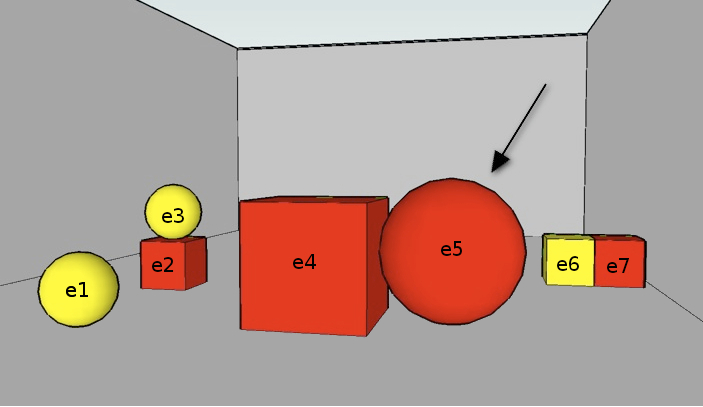
\includegraphics[width=.5\textwidth]{images/22.jpg}
%%\end{center}
%%\vspace*{-1.5em}
%%\caption{Escena 3D de figuras geom\'etricas}\label{figure22}
%%\end{figure}
%
%%\begin{figure}
%%\begin{minipage}[b]{0.6\linewidth}
%%\centering
%%\begin{tikzpicture}
%%  [
%%    n/.style={circle,fill,draw,inner sep=3pt,node distance=1.4cm},
%%    aArrow/.style={->, >=stealth, semithick, shorten <= 2pt, shorten >= 2pt},
%%  ]
%% \node[n,label=above:$e_1$,label=below:{
%%    \relsize{-1}$\begin{array}{c}
%%      \nLeft\\[-2pt]
%%      \nSmall\\[-2pt] 
%%      \nYellow \\[-2pt] 
%%      \nBall\end{array}$}] (a) {};
%
%% \node[n,label=above:$e_2$,label=below:{
%%    \relsize{-1}$\begin{array}{c}
%%      \nLeft\\[-2pt]
%%      \nSmall\\[-2pt] 
%%      \nRed\\[-2pt] 
%%      \nCube\end{array}$}, right of=a] (b) {};
%
%% \node[n,label=below:$e_3$,label=above:{
%%    \relsize{-1}$\begin{array}{c}
%%      \nTop\\[-2pt]
%%      \nLeft\\[-2pt]
%%      \nSmall\\[-2pt] 
%%      \nYellow\\[-2pt] 
%%      \nBall\end{array}$}, above of=b] (c) {};
%
%% \node[n,label=above:$e_4$,label=below:{
%%    \relsize{-1}$\begin{array}{c}
%%      \nBig\\[-2pt] 
%%      \nRed\\[-2pt] 
%%      \nCube\end{array}$}, right of=b] (d) {};
%
%% \node[n,label=above:$e_5$,label=below:{
%%    \relsize{-1}$\begin{array}{c}
%%      \nBig\\[-2pt] 
%%      \nRed\\[-2pt] 
%%      \nBall\end{array}$}, right of=d] (e) {};
%
%% \node[n,label=above:$e_6$,label=below:{
%%    \relsize{-1}$\begin{array}{c}
%%      \nSmall\\[-2pt] 
%%      \nYellow\\[-2pt] 
%%      \nCube\end{array}$}, right of=e] (f) {};
%
%% \node[n,label=above:$e_7$,label=below:{
%%    \relsize{-1}$\begin{array}{c}
%%      \nSmall\\[-2pt] 
%%      \nRed\\[-2pt] 
%%      \nCube\end{array}$}, right of=f] (g) {};
%
%% \draw [aArrow,bend right=90] (b) to node[auto,swap]{\relsize{-1}$\nBelow$} (c);
%% \draw [aArrow,bend right=90] (c) to node[auto,swap]{\relsize{-1}$\nOntop$} (b);
%
%% \draw [aArrow,bend right=30] (d) to node[auto,swap]{\relsize{-1}$\nLeftof$} (e);
%% \draw [aArrow,bend right=30] (e) to node[auto,swap]{\relsize{-1}$\nRightof$} (d);
%
%% \draw [aArrow,bend right=30] (f) to node[auto,swap]{\relsize{-1}$\nLeftof$} (g);
%% \draw [aArrow,bend right=30] (g) to node[auto,swap]{\relsize{-1}$\nRightof$} (f);
%
%% \draw[dotted] (-.4,-1.7) rectangle (7.5,3.3);
%
%% \end{tikzpicture}
%%\caption{La escena como modelo relacional}\label{GRE3D7-stimulus-graph}
%%\end{minipage}
%%\end{figure}
%
%
%El algoritmo siempre termina, y devuelve ER un conjunto de f\'ormulas que describe cada elemento en el dominio (si existe esa f\'ormula). \\
%
%En el comienzo ER=$\{\top\}$ y $\interp{\top}$ = $\{e_1, e_2, e_3, e_4, e_5, e_6, e_7\}$ como se puede ver en la Figura~\ref{fig-modelo}.\\
%
%ACA
%\begin{figure}[ht]
%\begin{minipage}[b]{0.45\linewidth}
%\centering
%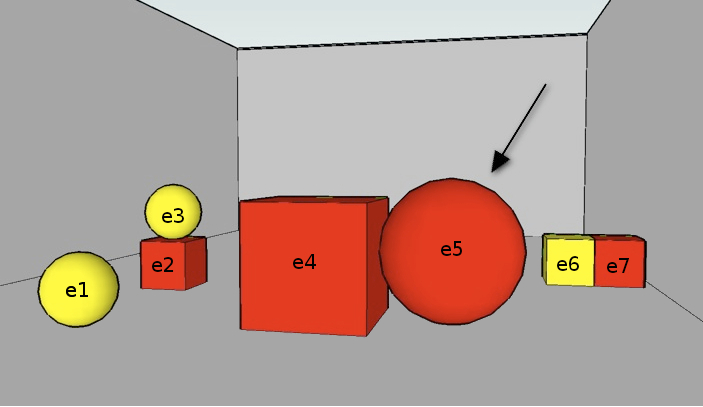
\includegraphics[width=\textwidth]{images/22.jpg}
%\vspace*{1cm}
%%\caption{Input scene}
%\label{GRE3D7-stimulus-22}
%\end{minipage}
%%\hspace*{-0.35cm}
%\begin{minipage}[b]{0.6\linewidth}
%\centering
%%\begin{figure}[ht]
%%\begin{center}
%\frame{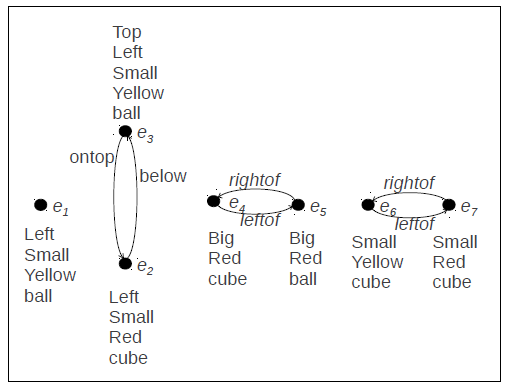
\includegraphics[width=8cm]{images/modelo.png}}\\[0pt]
%\caption{Modelo de la Figura \ref{GRE3D7-stimulus-22}}
%\label{fig-modelo}
%\end{minipage}
%\end{figure}
%El primer bucle del algoritmo es en las propiedades. Para cada propiedad hace add$_\el$ ($\varphi$, RE), las propiedades at\'omicas se muestran en la Figura~\ref{fig-modelo2}.
%
%\begin{figure}[ht]
%\begin{center}
%\frame{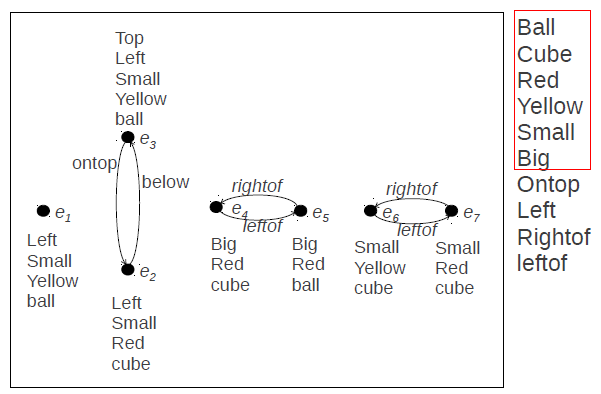
\includegraphics[width=8cm]{images/modelo2.png}}\\[0pt]
%\caption{Propiedades proposicionales en cuadro rojo, las del primer ciclo del algoritmo}
%\label{fig-modelo2}
%\end{center}
%\end{figure}
%
%La f\'ormula $\varphi$ se a\~nadir\'a a ER si su interpretaci\'on tiene al menos un elemento, a continuaci\'on, para cada f\'ormula
 %$\psi$ en ER la conjunci\'on
%$\varphi  \wedge \psi$ no necesita estar subsumida in ER, la $\interp{\varphi \cup \psi}$ no tiene que ser vac\'io, y su interpretaci\'on tiene que ser distinta de $\interp{\psi}$. Luego las f\'ormulas subsumidas se borran.
%
%La primer propiedad es \textsf{ball}, ER = \{$\top$, \textsf{ball}\}, se ven los elementos de ``ball'' en un recuadro en la Figura~\ref{fig-modelo3}.
%
%\begin{figure}[ht]
%\begin{center}
%\frame{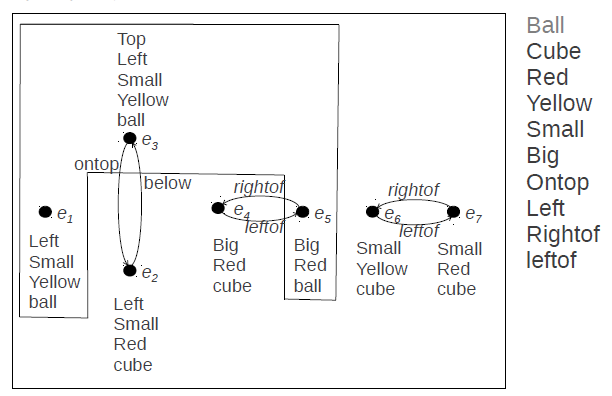
\includegraphics[width=8cm]{images/modelo3.png}}\\[0pt]
%\caption{El cuadro indica cuales son ``ball''}
%\label{fig-modelo3}
%\end{center}
%\end{figure}
%
%La siguiente propiedad es \textsf{cube}, ER = \{$\top$, \textsf{ball}, \textsf{cube}\}, pero ahora la $\interp{\textsf{ball}}$ = $\{e_1, e_3, e_5\}$, $\interp{\textsf{cube}}$ = $\{e_2, e_4, e_6, e_7\}$, quedando las particiones como se muestra en la Figura~\ref{fig-modelo4}
%\begin{figure}[ht]
%\begin{center}
%\frame{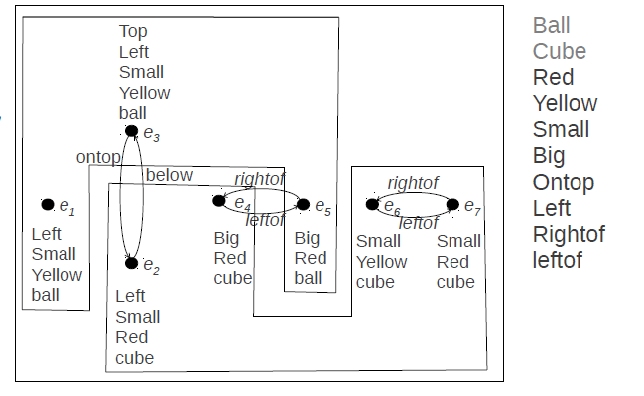
\includegraphics[width=8cm]{images/modelo4.png}}\\[0pt]
%\caption{Cuadros indicando ``ball'' y ``cube''}
%\label{fig-modelo4}
%\end{center}
%\end{figure}
%Ahora podemos borrar $\top$, porque es subsumida (esta cubierta por) las otras dos f\'ormulas. La siguiente propiedad es  \textsf{red}, $\interp{\textsf{red}}$ es: $\{e_2, e_4, e_5, e_7\}$, haciendo la intersecci\'on con la $\interp{.}$ de cada f\'ormula en ER obtenemos, $\{e_5\}$ y $\{e_2, e_4, e_7\}$, ER = $\{\textsf{ball}, \textsf{cube}, \textsf{ball} \wedge \textsf{red}, \textsf{cube} \wedge \textsf{red}\}$, las particiones actuales se pueden ver en la Figura~\ref{fig-modelo9}.
%\begin{figure}[ht]
%\begin{center}
%\frame{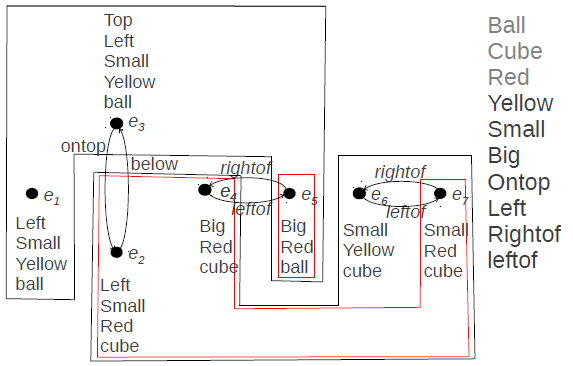
\includegraphics[width=8cm]{images/modelo9.png}}\\[0pt]
%\caption{Cuadros indicando ``ball'', ``cube'' y ``red''}
%\label{fig-modelo9}
%\end{center}
%\end{figure}
%
%Siguiendo con \textsf{yellow}, tenemos, $\interp{\textsf{yellow}}$ = $\{e_1, e_3, e_6\}$ y obtenemos ER = $\{\textsf{ball} \wedge \textsf{yellow}, \textsf{cube} \wedge \textsf{yellow}, \textsf{ball} \wedge \textsf{red}, \textsf{cube} \wedge \textsf{red}\}$. 
%Note que aqu\'i ya borramos la f\'ormula \textsf{ball} porque estaba subsumida, y la f\'ormula \textsf{cube} tambi\'en. Se muestran particiones en Figura~\ref{fig-modelo10}.
%
%\begin{figure}[ht]
%\begin{center}
%\frame{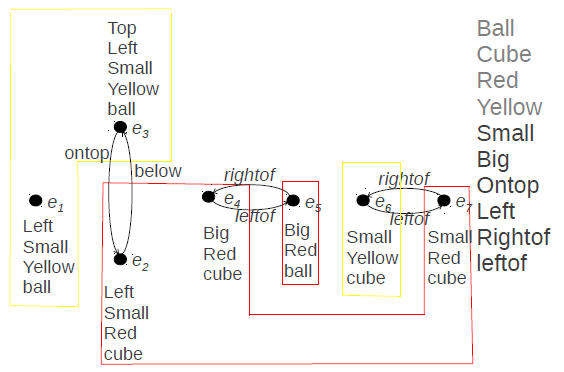
\includegraphics[width=8cm]{images/modelo10.png}}\\[0pt]
%\caption{Cuadros indicando ``ball'', ``cube'', ``red'' y ``yellow''}
%\label{fig-modelo10}
%\end{center}
%\end{figure}
%
%Haciendo lo mismo con \textsf{small} tenemos ER = $\{\textsf{ball} \wedge \textsf{yellow} \wedge \textsf{small}, \textsf{cube} \wedge \textsf{yellow} \wedge \textsf{small}, \textsf{ball} \wedge \textsf{red}, \textsf{cube} \wedge \textsf{red}, \textsf{cube} \wedge \textsf{red} \wedge \textsf{small}\}$, como se puede ver en Figura~\ref{fig-modelo11}.
%\begin{figure}[ht]
%\begin{center}
%\frame{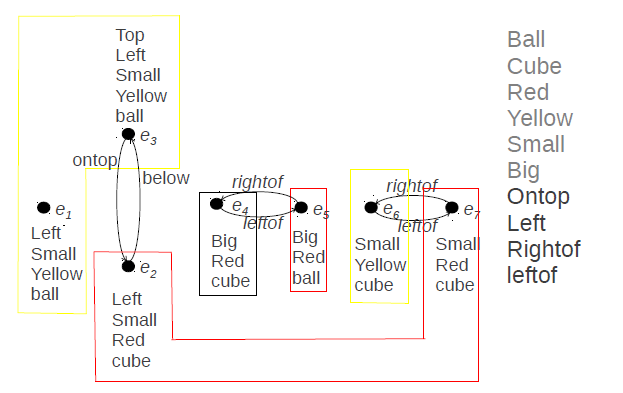
\includegraphics[width=8cm]{images/modelo11.png}}\\[0pt]
%\caption{Cuadros indicando ``ball'', ``cube'', ``red'', ``yellow'', ``small'' y ``large''}
%\label{fig-modelo11}
%\end{center}
%\end{figure}
%
%La siguiente propiedad es \textsf{large} as\'i, tenemos ER = $\{\textsf{ball} \wedge \textsf{yellow} \wedge \textsf{small}, \textsf{cube} \wedge \textsf{yellow} \wedge \textsf{small}, \textsf{ball} \wedge \textsf{red}, \textsf{cube} \wedge \textsf{red} \wedge \textsf{large}, \textsf{cube} \wedge \textsf{red} \wedge \textsf{small}\}$. Aqu\'i no podemos agregar \textsf{large} a la f\'ormula $\textsf{red} \wedge \textsf{cube}$ porque su interpretaci\'on tiene un solo elemento, y la condici\'on dice que es necesario tener m\'as de uno.
%
%Hasta ahora ER = $\{\textsf{ball} \wedge \textsf{yellow} \wedge \textsf{small}, \textsf{cube} \wedge \textsf{yellow} \wedge \textsf{small}, \textsf{ball} \wedge \textsf{red}, \textsf{cube} \wedge \textsf{red} \wedge \textsf{large}, \textsf{cube} \wedge \textsf{red} \wedge \textsf{small}\}$ 
%y tenemos las siguientes extensiones: $\{e_1, e_3\}, \{e_6\}, \{e_5\}, \{e_4\}, \{e_2, e_7\}$ respectivamente. 
%Hay dos f\'ormulas que a\'un pueden ser refinadas, $\textsf{ball} \wedge \textsf{yellow} \wedge \textsf{small}$ y $\textsf{cube} \wedge \textsf{red} \wedge \textsf{small}$ 
%debido a que tienen m\'as de un elemento cada una, por lo que entran en el ciclo, while del algoritmo 1, en la l\'inea 4. Ahora es el turno de las relaciones, la primera de ellas es \textsf{leftof}, para cada f\'ormula $\varphi$ en ER trataremos de hacer add$_\el$ ($\exists \textsf{leftof}.\varphi$, RE). Notar que $\psi$ solo puede ser $\textsf{ball} \wedge \textsf{yellow} \wedge \textsf{small}$ o $\textsf{cube} \wedge \textsf{red} \wedge \textsf{small}$ porque esos son los que su interpretaci\'on tiene m\'as de un elemento. 
%\begin{figure}[ht]
%\begin{center}
%\frame{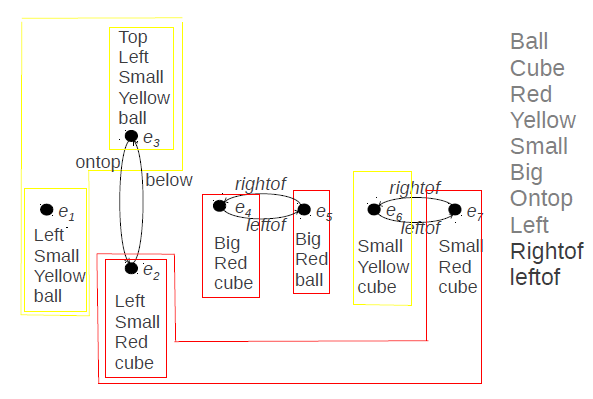
\includegraphics[width=8cm]{images/modelo15.png}}\\[0pt]
%\caption{Cuadros indicando ``ball'', ``cube'', ``red'', ``yellow''...}
%\label{fig-modelo15}
%\end{center}
%\end{figure}
%
%
%No hay
%%because those are the ones that its interpretation have more than one element. There is not 
%$\varphi$ y $\psi$ que puedan ser aplicadas. Continuando con \textsf{rightof} agregamos $\textsf{cube} \wedge \textsf{yellow} \wedge \textsf{small} \wedge \exists \textsf{rightof}. \textsf{cube} \wedge \textsf{red} \wedge \textsf{small}$, y asi con \textsf{topof} agregamos $\textsf{small} \wedge \textsf{red} \wedge \textsf{cube} \wedge \exists \textsf{ontop}. \textsf{small} \wedge \textsf{yellow} \wedge \textsf{ball}$ y el algoritmo termina con ER = $\{\textsf{ball} \wedge \textsf{yellow} \wedge \textsf{small}, \textsf{cube} \wedge \textsf{yellow} \wedge \textsf{small}, \textsf{ball} \wedge \textsf{red}, \textsf{cube} \wedge \textsf{red} \wedge \textsf{large}, \textsf{cube} \wedge \textsf{red} \wedge \textsf{small}, \textsf{cube} \wedge \textsf{yellow} \wedge \textsf{small} \wedge \exists \textsf{rightof}. \textsf{cube} \wedge \textsf{red} \wedge \textsf{small}, \textsf{small} \wedge \textsf{red} \wedge \textsf{cube} \wedge \exists \textsf{ontop}. \textsf{small} \wedge \textsf{yellow} \wedge \textsf{ball}\}$, 
%aqu\'i todos los elementos est\'an en una clase singleton y no se puede hacer ning\'un refinamiento m\'as. 
%%can be applied to $cube \wedge red \wedge small$ but there is no formula which interpretation has more than one element to be apply with this one. The same happen for the other relations, so the algorithm ends.
%%its interpretation is $\{e_7\}$ with $\psi$ is $cube \wedge yellow \wedge small$, the others combinations can't be apply because they don't do true the preconditions. The following relation is rightof, 
%
%%leftof, rightof, ontopof, bellowof
%
%%At this point we already have the target in a singleton set. So the formula for it is ``red and ball'', and also for s6 which formula is ``yellow cube''.\\
%%As we show this algorithm depends of the order of properties and relations.\\
%\begin{figure}[ht]
%\begin{center}
%\frame{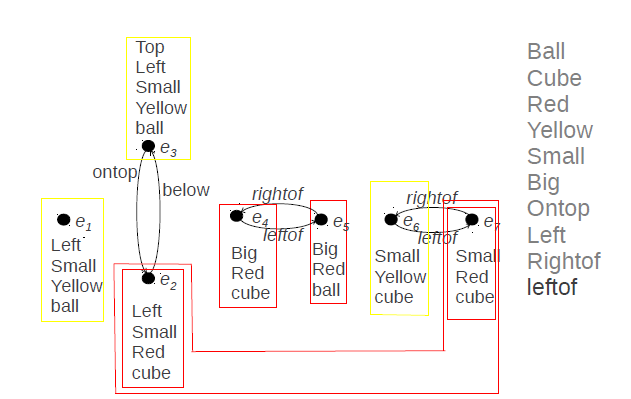
\includegraphics[width=8cm]{images/modelo16.png}}\\[0pt]
%\caption{Cuadros indicando ``ball'', ``cube'', ``red'', ``yellow''...}
%\label{fig-modelo16}
%\end{center}
%\end{figure}
%
%\begin{figure}[ht]
%\begin{center}
%\frame{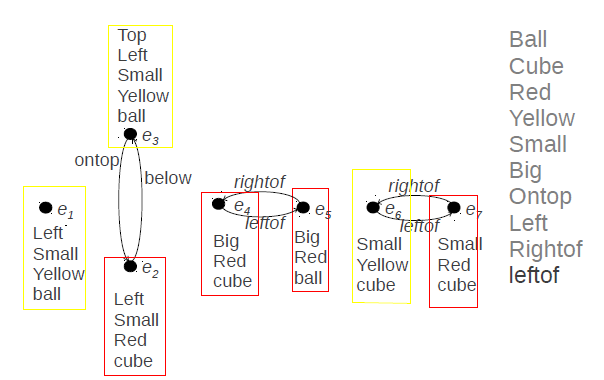
\includegraphics[width=8cm]{images/modelo17.png}}\\[0pt]
%\caption{Cuadros indicando ``ball'', ``cube'', ``red'', ``yellow''...}
%\label{fig-modelo17}
%\end{center}
%\end{figure}
%
%Las expresiones referenciales encontradas son:\\
%
%$\textsf{ball} \wedge \textsf{yellow} \wedge \textsf{small}$ representa $e_1$ \\
%$\textsf{cube} \wedge \textsf{yellow} \wedge \textsf{small}$ representa $e_6$ \\
%$\textsf{ball} \wedge \textsf{red}$ representa $e_5$ \\
%$\textsf{cube} \wedge \textsf{red} \wedge \textsf{large}$ representa $e_4$ \\
%$\textsf{cube} \wedge \textsf{red} \wedge \textsf{small}$ representa $\{e_2,e_7\}$  \\
%$\textsf{cube} \wedge \textsf{yellow} \wedge \textsf{small} \wedge \exists \textsf{rightof}. \textsf{cube} \wedge \textsf{red} \wedge \textsf{small}$ representa $e_6$ \\
%$\textsf{small} \wedge \textsf{red} \wedge \textsf{cube} \wedge \exists \textsf{ontop}. \textsf{small} \wedge \textsf{yellow} \wedge \textsf{ball}$ representa $e_2$ \\
%



%\section{Aproximaciones emp\'iricas a la soluci\'on de GER}
%\label{sec:trabajos_empiricos}
%
%
%
%
%\subsection{Trabajos emp\'iricos en el \'area}
%\label{sec:trab_emp}

%http://link.springer.com/chapter/10.1007/978-3-642-15573-4_9
%http://www.jetteviethen.net/papers/DaleViethen2010chapter.pdf



